%\VignetteIndexEntry{introduction}
\documentclass{article}

%%% latex packages
\usepackage[T1]{fontenc}
\usepackage{hyperref}
\usepackage[utf8]{inputenc}
\usepackage[usenames,dvipsnames]{xcolor}

\usepackage{lipsum} % for dummy text only

%% change margins to 1" all the way around
\oddsidemargin 0.0in
\evensidemargin 0.0in
\textwidth 6.5in
\headheight 0.0in
\topmargin 0.0in
\textheight 9.0in

%%% document info
\title{Introduction to \texttt{SpaDES}}

\author{
  Alex M. Chubaty\\
	\small{Natural Resources Canada, Pacific Forestry Centre}\\
	\small{email: \href{mailto:achubaty@nrcan.gc.ca}{achubaty@nrcan.gc.ca}}
	\and
	Eliot McIntire\\
	\small{Natural Resources Canada, Pacific Forestry Centre}\\
	\small{email: \href{mailto:emcintir@nrcan.gc.ca}{emcintir@nrcan.gc.ca}}
}

\usepackage{Sweave}
\begin{document}
\Sconcordance{concordance:introduction.tex:introduction.Rnw:%
1 31 1 1 0 14 1 1 3 2 0 1 1 1 10 8 0 1 2 7 0 1 5 14 1 1 2 1 0 4 1 1 2 4 %
0 1 2 22 1 1 2 1 0 1 4 2 0 1 2 1 0 3 1 1 5 3 0 1 1 1 2 11 0 1 1 15 0 1 %
7 5 0 1 2 5 0 1 2 7 1}

 % displays code as entered (no arranging lines)

\maketitle

\tableofcontents

\newpage

\section{Spatial Discrete Event Simulation (SpaDES)}

\subsection{Overview}

\paragraph{}
Why SpaDES exists

\begin{figure}[!htbp]
  \centering
	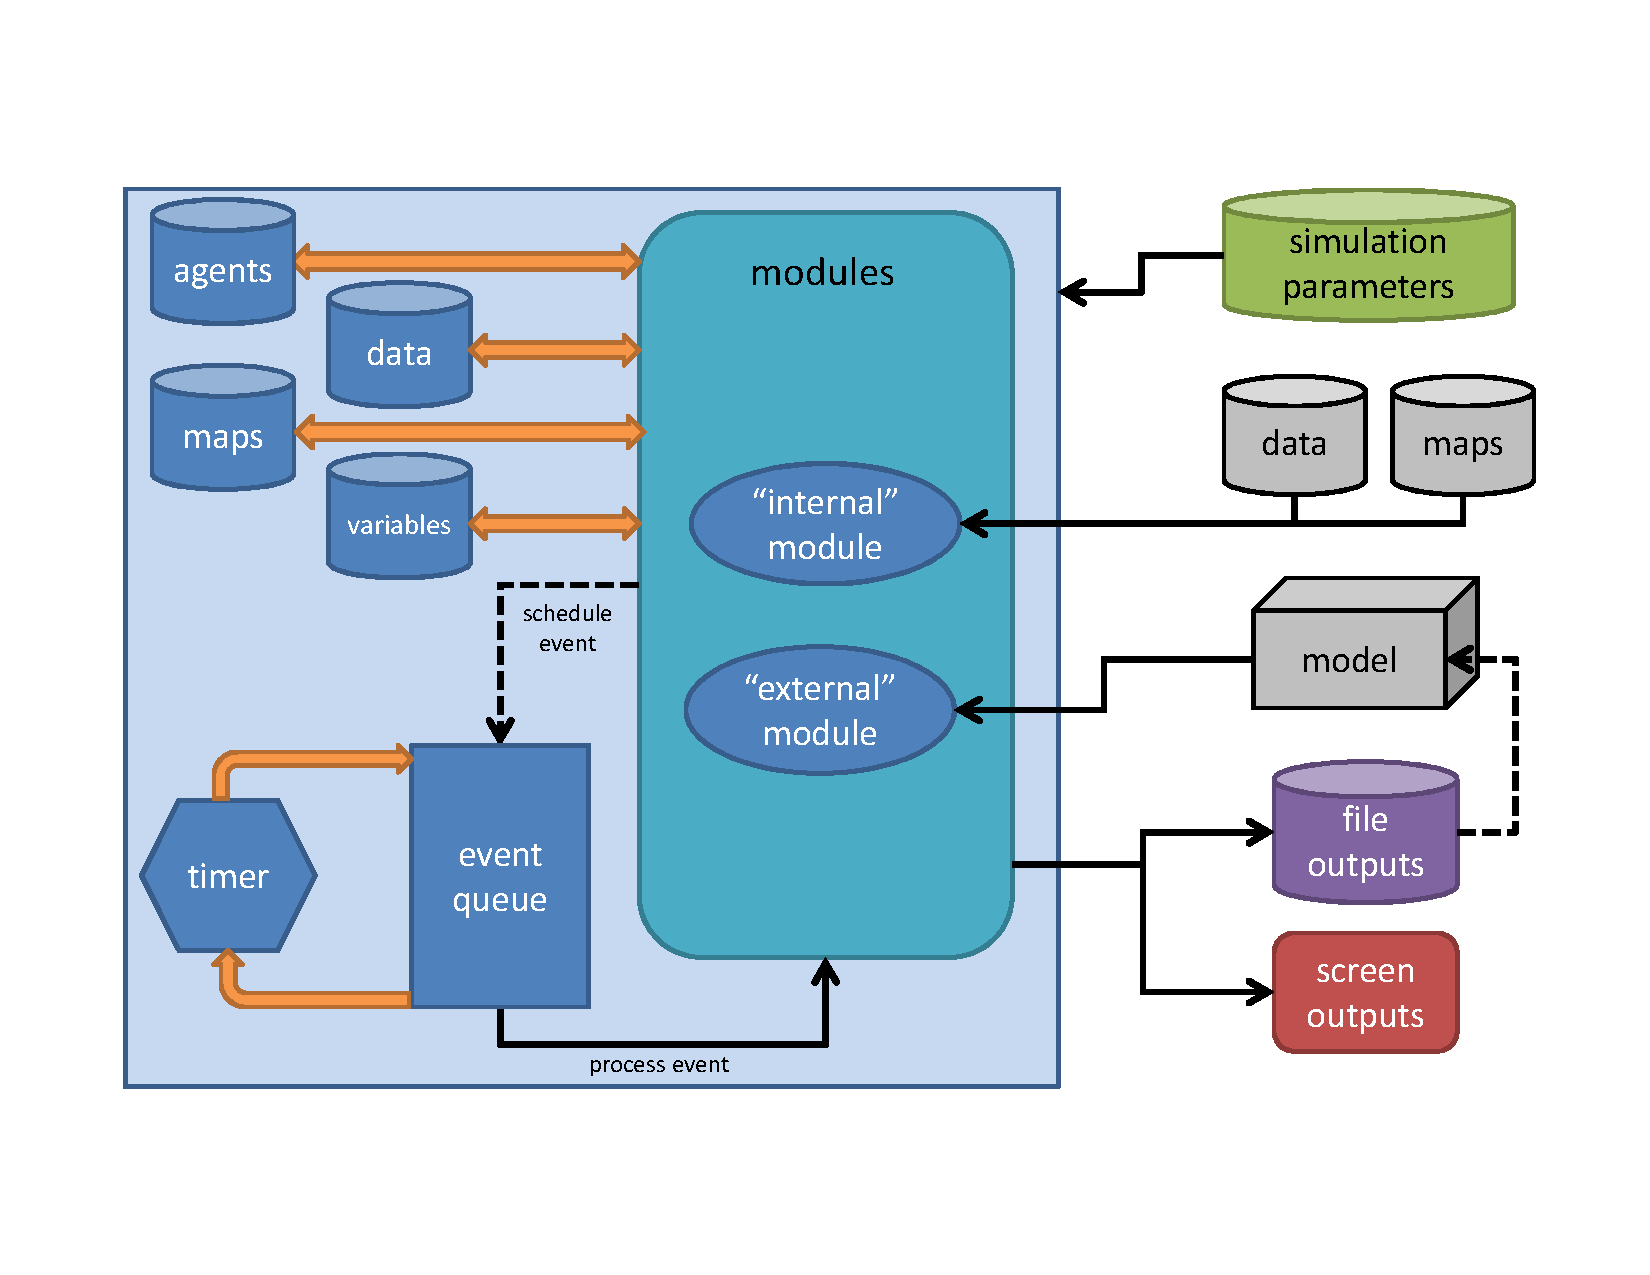
\includegraphics[width=5in]{../inst/SpaDES-overview-diagram.pdf}
	\caption{Schematic representation of a \texttt{SpaDES} simulation model.}
	\label{figure-SpaDES-overview}
\end{figure}

\subsection{What is Discrete Event Simulation}

\subsection{SpaDES is a DES}

